\chapter{Learned Probabilistic Sun Sensor}
\epigraph{He stepped down, avoiding any long look at her as one avoids long looks at the sun, but seeing her as one sees the sun, without looking.}{Leo Tolstoy, \textit{Anna Karenina}}
\label{ch:sun-bcnn}


\section{Background}
\subsection{Neural Networks for Parametric Learning}


\subsection{Convolutional Neural Networks}
\subsection{Regularization and Dropout}

\begin{figure}
\centering
\begin{subfigure}{0.45\textwidth}
	\centering
    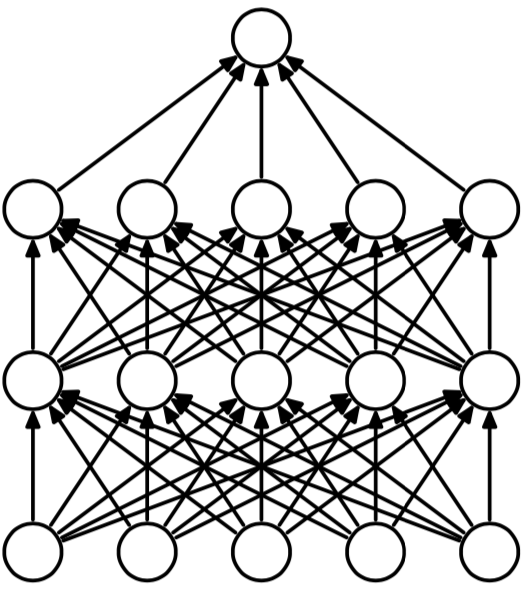
\includegraphics[width=0.8\textwidth]{sun-bcnn/dropout_fcn}
    \caption{Standard fully-connected neural network.}
\end{subfigure}
~
\begin{subfigure}{0.45\textwidth}
	\centering
    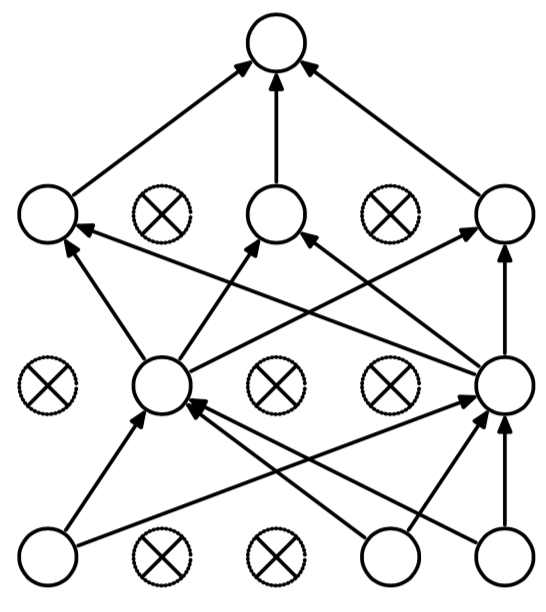
\includegraphics[width=0.8\textwidth]{sun-bcnn/dropout_fcnwdrop}
    \caption{A neural network with dropout applied.}
\end{subfigure}
\caption{The technique of \textit{dropout} stochastically removes the contribution of certain neurons to regularize learning. Figures	 from \cite{srivastava_dropout_2014}.}
\label{fig:sun-bcnn_dropout}
\end{figure}



\subsection{Dropout as Variational Inference}
\begin{align}
\label{eq:sun_direction_mean}
\Expectation{\Optimal{\Estimate{\SunDirection}}}_k &= \Optimal{\Estimate{\Mean{\SunDirection}}}_k \approx \frac{1}{N} \sum_{n=1}^N \Optimal{\Estimate{\SunDirection}}_k (\Optimal{\SunImage}_k, \CNNVariationalWeight^n) \\
\Expectation{\Optimal{\Estimate{\SunDirection}_k} \Transpose{\Optimal{\Estimate{\SunDirection}}}_k} &\approx \tau^{-1} \IdentityMatrix 
 +  \frac{1}{N} \sum_{n=1}^N \Optimal{\Estimate{\SunDirection}}_k(\Optimal{\SunImage}_k, \CNNVariationalWeight^n) \Transpose{\Optimal{\Estimate{\SunDirection}_k}(\Optimal{\SunImage}_k, \CNNVariationalWeight^n)} \notag \\ 
 &- \Optimal{\Estimate{\Mean{\SunDirection}}}_k \Transpose{\Optimal{\Estimate{\Mean{\SunDirection}}}_k},
 \label{eq:bcnn_covar}
\end{align}


